\documentclass[12pt,aspectratio=169]{beamer}
\usetheme{default}
\usecolortheme{dolphin}
\usefonttheme{structurebold}

\title{ShellScript 01}
\author{@aoirint}
\date{2020/04/16}
%\institute{}

\begin{document}

% 01
\frame{\maketitle}

% 02
\begin{frame}{テキスト}

  \begin{minipage}{0.58\textwidth}
    \begin{itemize}
      \item 新しいシェルプログラミングの教科書
      \begin{itemize}
        \item 著・三宅英明
        \item 刊・SB Creative
      \end{itemize}
    \end{itemize}

  \end{minipage}
  \hfill
  \begin{minipage}{0.38\textwidth}
    \vspace{-4\baselineskip}
    \begin{center}
      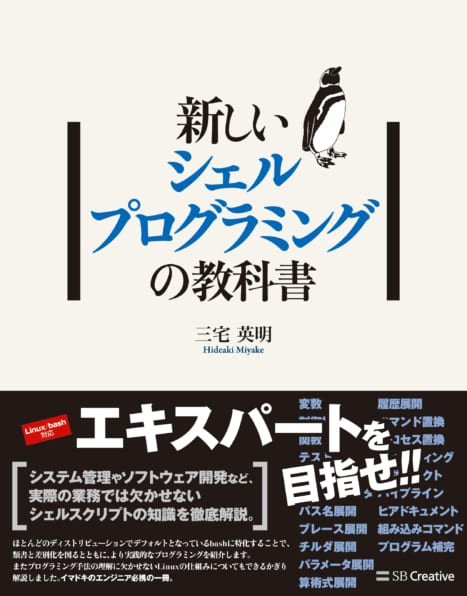
\includegraphics[width=5cm,bb=0 0 467 596]{./images/shellbook.jpg}
    \end{center}
  \end{minipage}

  \begin{itemize}
    \item 書影
    \begin{itemize}
      \item { \small \url{https://www.sbcr.jp/product/4797393101/} }
    \end{itemize}
  \end{itemize}

\end{frame}


\begin{frame}{シェルとは}


\end{frame}


\begin{frame}{Tips: Windows エクスプローラにコンテキストメニューを追加する}

\end{frame}

\begin{frame}{以上です}
てすと

\end{frame}


\end{document}
